\section{Introduction}
L'objectif du projet est d'implémenter un programme employant la stéganographie.\\\\
Dans le cadre du cours de Systèmes, la stéganographie nous permet d'approfondir l'utilisation de la mémoire pour stocker des informations. 
Nous devons apprendre en détail la structure des fichiers bitmaps et GIF pour pouvoir y cacher des messages. 
De plus, ce sujet nous permet d'approfondir le thème de la sécurité, un thème qui est fort lié aux systèmes d'exploitations.\\\\

Nous avons choisi d'implémenter 2 programmes en C qui cacheront un message à l'intérieur d'un bitmap et d'un GIF. 
Dans ce rapport, nous expliquerons pour chaque format la raison de notre choix, la technique utilisée, l'avancement du projet et un guide pour utiliser les executables. 


\section{Stéganographie : Définition}
La stéganographie est l'art de la dissimulation : son objet est de faire passer inaperçu un message dans un autre message. 
Elle se distingue de la cryptographie, « art du secret », qui cherche à rendre un message inintelligible à autre que qui-de-droit.\\


\section {Technique utilisée}
Pour cacher un message, nous employons la technique Least Significant Bit (LSB). \\

Comme vous le voyez sur le schéma ci-dessous, cette technique consiste à caché un bit d'information dans le bit le moins important d'un byte. 
Pour décripter le message, il suffit de lire le dernier bit de ces bytes et de reformer un message compréhensible.\\

Pour que le message ait le plus petit impact possible sur le fichier source, il faut employer des bytes qui peuvent perdre un bit d'information. 
Par exemple, pour une couleur codée en rgb, le changement du dernier bit a un impact très faible, quasi invisible à l'oeil nu.\\\\

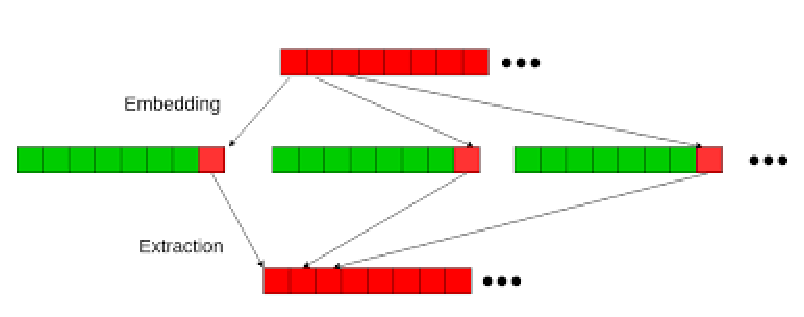
\includegraphics[width=12cm]{lsb.eps}\\


\section {Guide pratique}
Pour exécuter le projet, exécuter le makefile à la racine du fichier.
Voici quelques options possibles avec le makefile : \\
\lstinputlisting[language=make, firstline=1, lastline=18]{../makefile}